\subsection{Torben Bruhns}

\begin{wrapfigure}{L}{0.35\textwidth}
  \vspace{-20pt}
  \begin{center}
    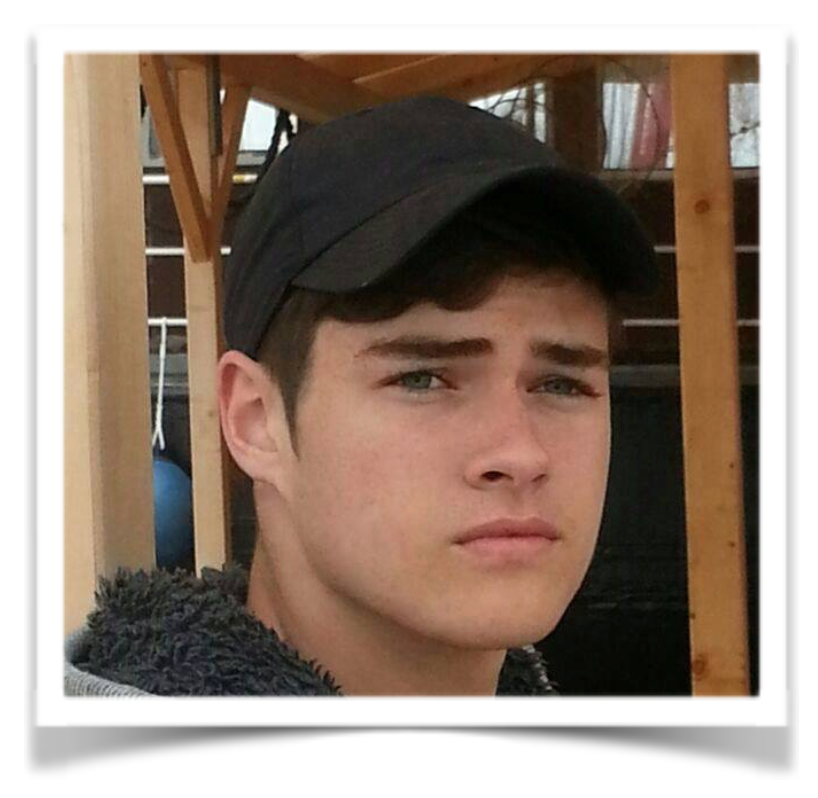
\includegraphics[width=0.32\textwidth]{./images/Torben_Bruhns}
  \end{center}
  \vspace{-40pt}
\end{wrapfigure}

\textbf{Name:} Torben Bruhns

\textbf{Alter:} 27

\textbf{Studium:} Informatik, 6. Semester

\textbf{Computerkenntnisse:} Sehr gut

\textbf{Ziele:} Bachelor- Abschluss schaffen durch so wenig Aufwand wie möglich 

\textbf{Vorlieben:} Computerspiele, Soziale Netzwerke, Aktive Benutzung komplizierter IDEs, Serien

\textbf{Motivation:} Interessiert sich für \texttt{ArguMens}, um den Dozenten fälschlicherweise von nicht existierendem Engangement zu überzeugen (Vortäuschen von aktiver Beteiligung).


